\subsection{Gruppe Arbejde}
\subsubsection{Organisering af gruppearbejde}

Som det første i projektet lavede vi en gruppekontrakt, 
hvori vi aftalte forholdene for dette projekt. Derefter udvekslede gruppen kontaktoplysninger.
I gruppekontakten aftalte vi alt fra mødetid til konflikthåndtering.


I kontrakten aftalte vi at vi ville bruge OneDrive til deling af filer, Trello som scrumboard, Discord til intern kommunikation, Lucidchart til vores artefakter og GitHub til versionsstyring. 
Endvidere aftalte vi også
at bruge Visual Studio som IDE.
Selve rapport blev skrevet i \LaTeX, da mange i gruppen havde haft en positiv oplevelse med det i tidligere projekter, og man kunne samtidig nemt tilføje og ændre ting i rapporten.

I gruppen lavede vi også en kvalitetsplan. Her blev vi alle tildelt nogle artefakter. 
Alle punkterne var så tildelt mellem gruppemedlemmerne. Alle de kvalitetspunkter man var givet var således ens ansvarsområde, som betød det var ens ansvar at sikre disse punkter var op til ordentlig kvalitet. 
Det betød ikke at det var en selv der skulle kvalitetssikre det, eller andre ikke kunne hjælpe til.

\subsubsection{Kontakt med virksomhed}

Undervejs i projektet havde vi kontakt med Psykolog Nord. Som vi undervejs har haft flere møder med, så vi kunne få deres input på udvikling af systemet.
Under disse møder har vi fået programmets krav bedre specificeret, samt fået inputs på hvorledes programmet kunne forbedres.

Vi fik etableret tidlig kontakt med vores virksomhed, da vi var tidlig ude og søge virksomhed. En af virksomhederne vi kom i kontakt med var så Psykolog Nord. vi mødtes med dem den 27 februar, hvor de uddybbede deres problem og vi afstemte forventninger. Projektet blev godkendt af underviserne, hvorefter vi aftalte et møde den 25 marts, før pre-sprinten, så problemet kunne blive specifikt, samt at Psykolog Nord kunne vise os deres problemstilling mere konkret, med centrale problemer opstillet.
Dertil aftalte vi de første møder i projektet. 

Vi havde så aftalt at holde møder med dem hver anden uge, hvor vi viste hvad vi havde nået, de kunne komme med input på programmet og vi kunne fået svar på spørgsmål som evt. var opstået under projektet. Dertil passede mødetiderne godt sammen med den planlagte længde for hver sprint. 
Vi måtte dog indse undervejs at vi ikke kunne nå at afslutte alt i vores sprints på 2 uger.

Møderne har hjulpet gevaldigt med at sikre udvikling i den rigtige retning, dertil fjernede de tvivler omkring den ønskede adfærd af systemet der opstod undervejs. 

\subsubsection{SCRUM og retrospektives}

Vi valgte at køre 2 ugers sprints, dette passede bedst med størrelserne af vores PBI'er og mødetiderne med vores PO ifht. sprintreviews.
I begyndelsen af hver sprint brugte vi planning poker til at vurdere hvor lang tid hver af de forskellige opgaver under sprinten ville tage.
Det gjorde det nemmere at se og vurdere vores fremskridt i sprintet, også selvom man nogen gange vurdere tidsforbruget på opgaven forkert.
Hver dag startede vi også ud med at fortælle hvad vi havde tænkt os at arbejde på i dag. Derved sikrede vi alle havde en opgave at gå i gang med.

Dertil hjalp det de næste sprints fremadrettet, da man så ved bedre hvor lang tid visse opgaver kræver.
Efter hvert sprint holdte vi et sprint retrospektiv. Her skiftede vi altid roller, så det ikke var den samme person der var SCRUM-master.
Efter hver uge i projektet kørte vi et happiness index for hver person.
Det havde vi internt i gruppen valgt at bruge, for at have en status over, hvordan folk syntes projektet gik, og om de havde evt. grunde til deres happiness.
Ens happiness, som gik på en skala 1-5, kunne være alt fra noget projektrelateret til bare hvorledes man havde det.

\begin{figure}[h]
    \caption{Graf for Happinessindex}
    \centering
        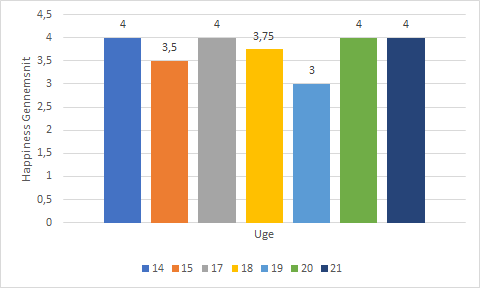
\includegraphics[width=\textwidth]{HappinessIndex.png}
    \label{happinessindex}
\end{figure}

Meget at tiden havde en positiv morale i gruppen. De eneste bemærkelsesværdige uger var uge 15 og uge 19.
I uge 15 var happinessen nede, da koncentrationen ikke var så stærk som i den tidligere uge. Dette forbedre sig efter.
I uge 19 var happinessen nede pga. vi fik besked på at undervisningsholdene vil blive splittet. Ud over det var alle meget tilfredse med arbejdet i projektet.


Under kodning gjorde vi stor brug af pairprogramming, dette hjalp med at mindske fejl, sikrede for bedre løsninger og gav os en større produktivitet.
Ud over dette aftalte vi i gruppen at efter noget er blevet lavet, 
skal det reviewes af et andet medlem i gruppen, før det kan kvalificeres som færdigt. Vi opholdte reglen ved at opsætte regler i Github, der gjorde det umuligt at lave et merge uden et pull-request.



\subsubsection{Erfaringer i projektet}

Undervejs har der opstået problemer i projektet. Et eksempel var da et gruppemedlem kom til at merge ind på masteren med en branch som ikke var up-to-date, hvilket betød meget af koden i masteren blev ændret. Heldigvis blev det indset med det samme og mergen blev reverted. På den måde fandt vi også ud af at vores Github regler var forkert sat op. Det blev så fikset.

Et mere alvorligt problem var da et gruppemedlem manglede filer efter at have mergede to branches. I forsøget på at løse dette problem mistede begge branches kode, som så skulle genskrives. Heldigvis var koden skrevet på samme dag, så da de manglende dele var fundet var det ikke for svært at skrive igen. Hertil lærte vi så at Github ikke cloner alt med hver eneste gang du henter en branch ned. Derimod ved vi nu at det altid er en god ide at rebuild en solution.